\documentclass[a4paper,10pt]{report}
\usepackage[utf8]{inputenc}
\usepackage{hyperref}
\nofiles
\usepackage{graphicx}
% Title Page
\title{Dossier Technique\\ Extension Web}
\author{THIVEND Baptiste}


\begin{document}
\maketitle

\begin{abstract}
 Créer une extension web capable de rediriger les utilisateurs vers les différentes parties du site i-boycott.org. Il existera deux versions : version non-connectée et version connectée (avec connexion possible et système de notification. La diversité des navigateurs web nous pousse à développer ces applications pour Google Chrome, Chromium, Firefox, Safari et Opera.
\begin{figure}[h]
\begin{center}
  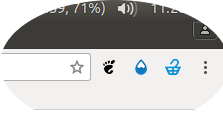
\includegraphics{apercu.png}
 \caption{Rendu dans la barre de recherche d'un navigateur}
\end{center}
\end{figure}

 \end{abstract}

\part{Développement}
\section{Version non-connectée}
On développera l'application sous Chrome, et les fichiers seront écrits sous Sublimetext, Atom, ou tout éditeur de texte faisant l'affaire.
\subsection{Création du dossier de l'extension}
Ce dernier contiendra les données nécessaire à l'exécution de l'application.
Structure minimale:

\begin{enumerate}
 \item le fichier \textbf{manifest.json} avec son icône
 \item le fichier \textbf{popup.html} et les fichiers rattachés(fichier CSS, fichiers Js, images, polices,...)
\end{enumerate}

\subsection{manifest.json}
Structure: code à recopier tel quel en modifiant les noms et descriptions selon les fichiers utilisés
\begin{verbatim}
  {
	"manifest_version":2,
	"name":"i-boycott", 								
	"description":"Permet de se tenir au courant des actualités I-boycott",		
	"version":"1.0",								

	"browser_action":{								
		"default_icon":"icon.png",						
		"default_popup":"popup.html"						
	}

}
\end{verbatim}
\begin{itemize}
 \item Ne pas oublier de mettre le fichier \textbf{icon.png} dans le dossier de l'extension: ce sera l'icône de l'extension dans la barre de recherche
\end{itemize}

\subsection{popup.html}
Ecrit en HTML5, il décrit le fonctionnement de l'extension: liens, images, textes. On me mets en forme grâce à un fichier CSS externe (par exemple popup.css) placé dans le même dossier.
On peut égaler rajouter du code Javascript. L'essentiel est tous les éléments utilisés (images, fichiers externes) soient correctement référencés pour la bonne éxécution du script.

\section{Version connectée}


\part{Déploiement}

Le protocole est le même à chaque fois:
\begin{itemize}
 \item Tester l'extension localement et procéder aux ajustements nécessaires
 \item Se créer un compte navigateur
 \item Mettre en ligne l'application
\end{itemize}


\section{Google Chrome et Chromium}
\begin{enumerate}
 \item Tester l'application non empaquetée via \url{chrome://extensions/}
 \begin{figure}[h]
  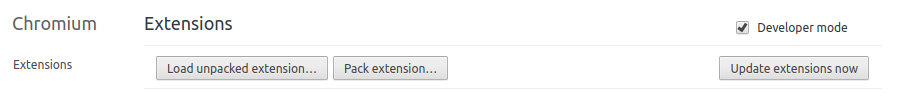
\includegraphics[scale=0.5]{test_chrome.png}
 \end{figure}
  \item Se créer un compte Google
 \item Se rendre sur le site \url{https://chrome.google.com/webstore/category/extensions}
 \item Dans les paramètres, aller sur \textbf{Developer Tools/Developer Dashboard}
 \begin{figure}[h]
 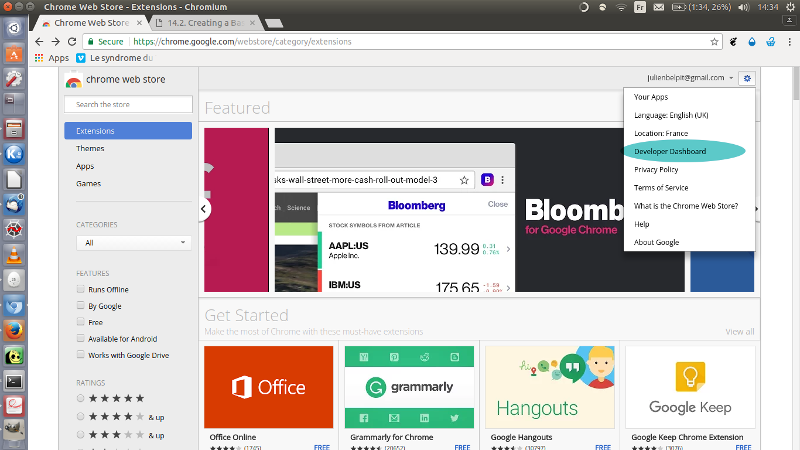
\includegraphics[scale=0.5]{chrome.png}
 \caption{Mode de développement Chrome}
\end{figure}
 \item Suivre les instructions pour mettre en ligne l'application, à remarquer que la publication est payante (5\$ en juillet 2017)
\end{enumerate}





\section{Firefox}
\begin{enumerate}

 \item Tester l'extension en utilisant \url{about:debugging} et en chargeant le dossier créée pour Chrome. Faire les modifications qui s'impose en modifiant les fichiers de l'extension dans un nouveau répertoire.
 \begin{figure}[h!]
  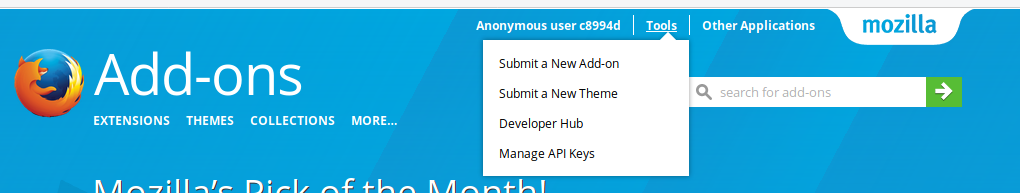
\includegraphics[scale=0.2]{test_firefox.png}
  \caption{Test de l'extension sur Firefox}
 \end{figure}
 \item Se créer un compte sur Mozilla
 \item Se rendre sur le site \url{https://addons.mozilla.org/en-US/firefox/} et suivre les instructions.
\begin{figure}[h]
 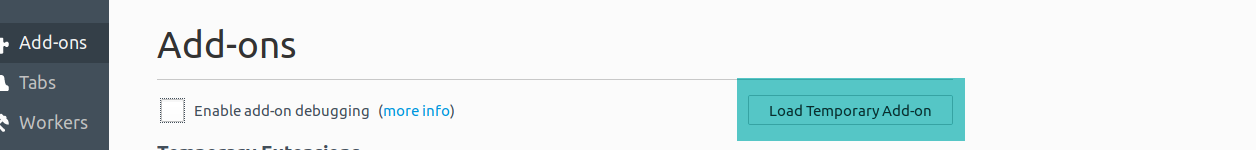
\includegraphics[scale=0.5]{firefox.png}
 \caption{Mode de développement Firefox}
\end{figure}
 \item Publier une extension sous Firefox est \textbf{gratuit}
\end{enumerate}





\section{Safari}

Il est nécessaire de posséder un appareil de la marque Apple pour publier une extension Safari!
\begin{enumerate}
 \item Se créer un compte Safari
 \item Se rendre sur le site \url{https://developer.apple.com/safari/}
 \item Suivre les instructions
\end{enumerate}





\section{Opera}
\begin{enumerate}
 \item Se créer un compte Opéra
 \item Se rendre sur \url{https://addons.opera.com/developer/}
 \item Suivre les instructions
\end{enumerate}

\end{document}          
